\documentclass[tikz,border=6pt]{standalone}
\usepackage[utf8]{inputenc}
\usepackage{amsmath,amssymb}
\usetikzlibrary{arrows.meta, positioning, calc}
\renewcommand{\familydefault}{\sfdefault}

\begin{document}
	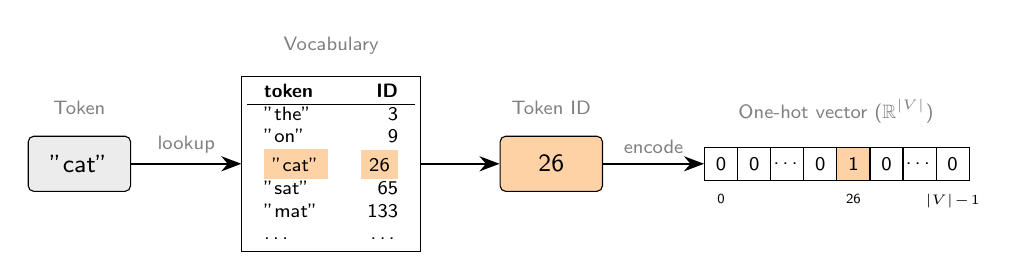
\begin{tikzpicture}[
		font=\sffamily\small,
		arrow/.style={-{Stealth[scale=1.1]}, thick},
		lbl/.style={font=\sffamily\scriptsize, text=gray},
		tok/.style={rectangle, rounded corners=2pt, draw=black, fill=gray!15, minimum height=0.7cm, minimum width=1.3cm},
		cell/.style={rectangle, draw=black, minimum size=0.42cm, inner sep=0pt, font=\sffamily\scriptsize}
		]
		
		% 1. Token
		\node[tok] (token) {"cat"};
		\node[lbl, above=0.15cm of token] {Token};
		
		% 2. Vocabulary (lookup table)
		\node[right=1.4cm of token, draw=black, inner sep=2pt] (vocab) {
			\scriptsize
			\begin{tabular}{lr}
				\textbf{token} & \textbf{ID} \\
				\hline
				"the" & 3 \\
				"on"  & 9 \\
				\colorbox{orange!35}{"cat"} & \colorbox{orange!35}{26} \\
				"sat" & 65 \\
				"mat" & 133 \\
				\dots & \dots
			\end{tabular}
		};
		\node[lbl, above=0.15cm of vocab] {Vocabulary};
		
		% 3. Integer ID
		\node[tok, right=1.0cm of vocab, fill=orange!35] (id) {26};
		\node[lbl, above=0.15cm of id] {Token ID};
		
		% 4. One-hot vector of size |V|
		\begin{scope}[shift={($(id.east)+(1.5cm,0)$)}]
			\foreach \v [count=\k from 0] in {0,0,\dots,0,1,0,\dots,0} {
				\ifnum\k=4
				\node[cell, fill=orange!35] (c\k) at (\k*0.42, 0) {\v};
				\else
				\node[cell] (c\k) at (\k*0.42, 0) {\v};
				\fi
			}
			\node[font=\sffamily\tiny, below=0.05cm of c0] {0};
			\node[font=\sffamily\tiny, below=0.05cm of c4] {26};
			\node[font=\sffamily\tiny, below=0.05cm of c7] {$|V|\!-\!1$};
		\end{scope}
		\node[lbl] at ($(c3.north)+(0.2,0.45)$) {One-hot vector ($\mathbb{R}^{|V|}$)};
		
		% Arrows
		\draw[arrow] (token) -- node[above, lbl] {lookup} (vocab);
		\draw[arrow] (vocab) -- (id);
		\draw[arrow] (id) -- node[above, lbl] {encode} (c0.west);
	\end{tikzpicture}
\end{document}